%% Supplementary Materials IEEE OJEMB

\documentclass[journal]{IEEEtran}
\usepackage[usenames]{color}
\usepackage{epsfig}
\usepackage{graphics}
\usepackage{caption}
\usepackage{amsmath}
\usepackage{amssymb}
\usepackage{multirow}
\usepackage{cite}
\usepackage{array}
\usepackage{pslatex} 
\usepackage{url}
\usepackage{lineno}
\usepackage{graphicx}  % Written by David Carlisle and Sebastian Rahtz
\usepackage{setspace}
\usepackage{tikz}
\usepackage{hhline}
\usepackage{mathtools}
\usepackage{caption}
\usepackage[letterpaper]{geometry}
\geometry{verbose,tmargin=0.7in,bmargin=0.7in,lmargin=0.65in,rmargin=0.65in}
\setlength{\headheight}{17pt}
\setlength{\headsep}{5pt}
%\captionsetup{labelfont={up},font=small}
\captionsetup[figure]{name={Fig.},labelsep=period,font=small}
 \captionsetup[table]{name={TABLE},labelsep=period,font=small}
% If IEEEtran.cls has not been installed into the LaTeX system files,
% manually specify the path to it like:
% \documentclass[journal]{../sty/IEEEtran}

\usepackage{lipsum}

\usepackage{soul}
\newcommand{\etal}{\textit{et al}., }
\newcommand{\ie}{\textit{i}.\textit{e}., }
\newcommand{\eg}{\textit{e}.\textit{g}.\ }
\newcommand{\cf}{\textit{cf}.\ }
\usepackage{hyperref}


% Some very useful LaTeX packages include:
% (uncomment the ones you want to load)


% *** MISC UTILITY PACKAGES ***
%
%\usepackage{ifpdf}
% Heiko Oberdiek's ifpdf.sty is very useful if you need conditional
% compilation based on whether the output is pdf or dvi.
% usage:
% \ifpdf
%   % pdf code
% \else
%   % dvi code
% \fi
% The latest version of ifpdf.sty can be obtained from:
% http://www.ctan.org/pkg/ifpdf
% Also, note that IEEEtran.cls V1.7 and later provides a builtin
% \ifCLASSINFOpdf conditional that works the same way.
% When switching from latex to pdflatex and vice-versa, the compiler may
% have to be run twice to clear warning/error messages.






% *** CITATION PACKAGES ***
%
%\usepackage{cite}
% cite.sty was written by Donald Arseneau
% V1.6 and later of IEEEtran pre-defines the format of the cite.sty package
% \cite{} output to follow that of the IEEE. Loading the cite package will
% result in citation numbers being automatically sorted and properly
% "compressed/ranged". e.g., [1], [9], [2], [7], [5], [6] without using
% cite.sty will become [1], [2], [5]--[7], [9] using cite.sty. cite.sty's
% \cite will automatically add leading space, if needed. Use cite.sty's
% noadjust option (cite.sty V3.8 and later) if you want to turn this off
% such as if a citation ever needs to be enclosed in parenthesis.
% cite.sty is already installed on most LaTeX systems. Be sure and use
% version 5.0 (2009-03-20) and later if using hyperref.sty.
% The latest version can be obtained at:
% http://www.ctan.org/pkg/cite
% The documentation is contained in the cite.sty file itself.






% *** GRAPHICS RELATED PACKAGES ***
%
\ifCLASSINFOpdf
  % \usepackage[pdftex]{graphicx}
  % declare the path(s) where your graphic files are
  % \graphicspath{{../pdf/}{../jpeg/}}
  % and their extensions so you won't have to specify these with
  % every instance of \includegraphics
  % \DeclareGraphicsExtensions{.pdf,.jpeg,.png}
\else
  % or other class option (dvipsone, dvipdf, if not using dvips). graphicx
  % will default to the driver specified in the system graphics.cfg if no
  % driver is specified.
  % \usepackage[dvips]{graphicx}
  % declare the path(s) where your graphic files are
  % \graphicspath{{../eps/}}
  % and their extensions so you won't have to specify these with
  % every instance of \includegraphics
  % \DeclareGraphicsExtensions{.eps}
\fi
% graphicx was written by David Carlisle and Sebastian Rahtz. It is
% required if you want graphics, photos, etc. graphicx.sty is already
% installed on most LaTeX systems. The latest version and documentation
% can be obtained at: 
% http://www.ctan.org/pkg/graphicx
% Another good source of documentation is "Using Imported Graphics in
% LaTeX2e" by Keith Reckdahl which can be found at:
% http://www.ctan.org/pkg/epslatex
%
% latex, and pdflatex in dvi mode, support graphics in encapsulated
% postscript (.eps) format. pdflatex in pdf mode supports graphics
% in .pdf, .jpeg, .png and .mps (metapost) formats. Users should ensure
% that all non-photo figures use a vector format (.eps, .pdf, .mps) and
% not a bitmapped formats (.jpeg, .png). The IEEE frowns on bitmapped formats
% which can result in "jaggedy"/blurry rendering of lines and letters as
% well as large increases in file sizes.
%
% You can find documentation about the pdfTeX application at:
% http://www.tug.org/applications/pdftex





% *** MATH PACKAGES ***
%
\usepackage{amsmath}
% A popular package from the American Mathematical Society that provides
% many useful and powerful commands for dealing with mathematics.
%
% Note that the amsmath package sets \interdisplaylinepenalty to 10000
% thus preventing page breaks from occurring within multiline equations. Use:
%\interdisplaylinepenalty=2500
% after loading amsmath to restore such page breaks as IEEEtran.cls normally
% does. amsmath.sty is already installed on most LaTeX systems. The latest
% version and documentation can be obtained at:
% http://www.ctan.org/pkg/amsmath





% *** SPECIALIZED LIST PACKAGES ***
%
\usepackage{algorithmic}
% algorithmic.sty was written by Peter Williams and Rogerio Brito.
% This package provides an algorithmic environment fo describing algorithms.
% You can use the algorithmic environment in-text or within a figure
% environment to provide for a floating algorithm. Do NOT use the algorithm
% floating environment provided by algorithm.sty (by the same authors) or
% algorithm2e.sty (by Christophe Fiorio) as the IEEE does not use dedicated
% algorithm float types and packages that provide these will not provide
% correct IEEE style captions. The latest version and documentation of
% algorithmic.sty can be obtained at:
% http://www.ctan.org/pkg/algorithms
% Also of interest may be the (relatively newer and more customizable)
% algorithmicx.sty package by Szasz Janos:
% http://www.ctan.org/pkg/algorithmicx




% *** ALIGNMENT PACKAGES ***
%
\usepackage{array}
% Frank Mittelbach's and David Carlisle's array.sty patches and improves
% the standard LaTeX2e array and tabular environments to provide better
% appearance and additional user controls. As the default LaTeX2e table
% generation code is lacking to the point of almost being broken with
% respect to the quality of the end results, all users are strongly
% advised to use an enhanced (at the very least that provided by array.sty)
% set of table tools. array.sty is already installed on most systems. The
% latest version and documentation can be obtained at:
% http://www.ctan.org/pkg/array


% IEEEtran contains the IEEEeqnarray family of commands that can be used to
% generate multiline equations as well as matrices, tables, etc., of high
% quality.




% *** SUBFIGURE PACKAGES ***
%\ifCLASSOPTIONcompsoc
%  \usepackage[caption=false,font=normalsize,labelfont=sf,textfont=sf]{subfig}
%\else
%  \usepackage[caption=false,font=footnotesize]{subfig}
%\fi
% subfig.sty, written by Steven Douglas Cochran, is the modern replacement
% for subfigure.sty, the latter of which is no longer maintained and is
% incompatible with some LaTeX packages including fixltx2e. However,
% subfig.sty requires and automatically loads Axel Sommerfeldt's caption.sty
% which will override IEEEtran.cls' handling of captions and this will result
% in non-IEEE style figure/table captions. To prevent this problem, be sure
% and invoke subfig.sty's "caption=false" package option (available since
% subfig.sty version 1.3, 2005/06/28) as this is will preserve IEEEtran.cls
% handling of captions.
% Note that the Computer Society format requires a larger sans serif font
% than the serif footnote size font used in traditional IEEE formatting
% and thus the need to invoke different subfig.sty package options depending
% on whether compsoc mode has been enabled.
%
% The latest version and documentation of subfig.sty can be obtained at:
% http://www.ctan.org/pkg/subfig




% *** FLOAT PACKAGES ***
%
%\usepackage{fixltx2e}
% fixltx2e, the successor to the earlier fix2col.sty, was written by
% Frank Mittelbach and David Carlisle. This package corrects a few problems
% in the LaTeX2e kernel, the most notable of which is that in current
% LaTeX2e releases, the ordering of single and double column floats is not
% guaranteed to be preserved. Thus, an unpatched LaTeX2e can allow a
% single column figure to be placed prior to an earlier double column
% figure.
% Be aware that LaTeX2e kernels dated 2015 and later have fixltx2e.sty's
% corrections already built into the system in which case a warning will
% be issued if an attempt is made to load fixltx2e.sty as it is no longer
% needed.
% The latest version and documentation can be found at:
% http://www.ctan.org/pkg/fixltx2e


%\usepackage{stfloats}
% stfloats.sty was written by Sigitas Tolusis. This package gives LaTeX2e
% the ability to do double column floats at the bottom of the page as well
% as the top. (e.g., "\begin{figure*}[!b]" is not normally possible in
% LaTeX2e). It also provides a command:
%\fnbelowfloat
% to enable the placement of footnotes below bottom floats (the standard
% LaTeX2e kernel puts them above bottom floats). This is an invasive package
% which rewrites many portions of the LaTeX2e float routines. It may not work
% with other packages that modify the LaTeX2e float routines. The latest
% version and documentation can be obtained at:
% http://www.ctan.org/pkg/stfloats
% Do not use the stfloats baselinefloat ability as the IEEE does not allow
% \baselineskip to stretch. Authors submitting work to the IEEE should note
% that the IEEE rarely uses double column equations and that authors should try
% to avoid such use. Do not be tempted to use the cuted.sty or midfloat.sty
% packages (also by Sigitas Tolusis) as the IEEE does not format its papers in
% such ways.
% Do not attempt to use stfloats with fixltx2e as they are incompatible.
% Instead, use Morten Hogholm'a dblfloatfix which combines the features
% of both fixltx2e and stfloats:
%
% \usepackage{dblfloatfix}
% The latest version can be found at:
% http://www.ctan.org/pkg/dblfloatfix




%\ifCLASSOPTIONcaptionsoff
%  \usepackage[nomarkers]{endfloat}
% \let\MYoriglatexcaption\caption
% \renewcommand{\caption}[2][\relax]{\MYoriglatexcaption[#2]{#2}}
%\fi
% endfloat.sty was written by James Darrell McCauley, Jeff Goldberg and 
% Axel Sommerfeldt. This package may be useful when used in conjunction with 
% IEEEtran.cls'  captionsoff option. Some IEEE journals/societies require that
% submissions have lists of figures/tables at the end of the paper and that
% figures/tables without any captions are placed on a page by themselves at
% the end of the document. If needed, the draftcls IEEEtran class option or
% \CLASSINPUTbaselinestretch interface can be used to increase the line
% spacing as well. Be sure and use the nomarkers option of endfloat to
% prevent endfloat from "marking" where the figures would have been placed
% in the text. The two hack lines of code above are a slight modification of
% that suggested by in the endfloat docs (section 8.4.1) to ensure that
% the full captions always appear in the list of figures/tables - even if
% the user used the short optional argument of \caption[]{}.
% IEEE papers do not typically make use of \caption[]'s optional argument,
% so this should not be an issue. A similar trick can be used to disable
% captions of packages such as subfig.sty that lack options to turn off
% the subcaptions:
% For subfig.sty:
% \let\MYorigsubfloat\subfloat
% \renewcommand{\subfloat}[2][\relax]{\MYorigsubfloat[]{#2}}
% However, the above trick will not work if both optional arguments of
% the \subfloat command are used. Furthermore, there needs to be a
% description of each subfigure *somewhere* and endfloat does not add
% subfigure captions to its list of figures. Thus, the best approach is to
% avoid the use of subfigure captions (many IEEE journals avoid them anyway)
% and instead reference/explain all the subfigures within the main caption.
% The latest version of endfloat.sty and its documentation can obtained at:
% http://www.ctan.org/pkg/endfloat
%
% The IEEEtran \ifCLASSOPTIONcaptionsoff conditional can also be used
% later in the document, say, to conditionally put the References on a 
% page by themselves.




% *** PDF, URL AND HYPERLINK PACKAGES ***
%
\usepackage{url}
% url.sty was written by Donald Arseneau. It provides better support for
% handling and breaking URLs. url.sty is already installed on most LaTeX
% systems. The latest version and documentation can be obtained at:
% http://www.ctan.org/pkg/url
% Basically, \url{my_url_here}.




% *** Do not adjust lengths that control margins, column widths, etc. ***
% *** Do not use packages that alter fonts (such as pslatex).         ***
% There should be no need to do such things with IEEEtran.cls V1.6 and later.
% (Unless specifically asked to do so by the journal or conference you plan
% to submit to, of course. )

\usepackage{siunitx}
\sisetup{parse-numbers = false}
\usepackage{placeins}

\newcommand{\flogo}{
\includegraphics[height=18pt]{embLogo.eps}}



%\lhead{\textsc{\flogo}}
 
% The paper headers
\usepackage[english]{babel}
\usepackage[utf8]{inputenc}
\usepackage{setspace}
\usepackage{fancyhdr}
\pagestyle{fancy}
\fancyhf{}
\lhead{\textsc{\flogo}}
\rhead{\textcolor{violet}{\Large\textbf{Supplementary Materials}}}
\fancyfoot[C]{\thepage}
\renewcommand{\footrulewidth}{0.4pt}% default is 0pt

\begin{document}

\twocolumn[
\begin{@twocolumnfalse}
\thispagestyle{fancy}   
\vspace*{0.5cm}
\textbf{\LARGE{Supplementary Materials}}\\
\\
\medskip\Large{Compressed Sensing for Characterization of Tinnitus}\\
\normalsize{ Alec Hoyland,
	Nelson Barnett, Benjamin W. Roop, Adam C. Lammert}\\
	\vspace*{0.5cm}
\end{@twocolumnfalse}
]	


	

% make the title area





\IEEEPARstart{T}his document contains a description of additional experiments to find a performant
stimulus generation method and a discussion of sparsity in tinnitus signals.
The code for all experiments is freely available at \url{https://github.com/alec-hoyland/tinnitus-project}
and the data are available upon request.

\section{Stimulus Generation}

In the context of this paper, a stimulus generation method
is a process that generates a random waveform that is:

\begin{enumerate}
  \item auditorally-distinguishable
  \item statistically uncorrelated, and
  \item similar to tinnitus percepts.
\end{enumerate}

Additionally, compressed sensing requires that the matrix of stimuli
should satisfy the restricted isometry property,
which many random matrices do with high probability (\eg Gaussian random matrices)
\cite{candesRestrictedIsometryProperty2008,candesIntroductionCompressiveSampling2008}.

\subsection{Auditorally-Distinguishable Stimuli}

We used mel-frequency binning to ensure that our stimuli were auditorally-distinguishable.
The mel scale is a perceptual scale of pitches judged by listeners to be equal in distance
from one to another (Fig. \ref{fig:hz2mel}) \cite{hamiltonTopographySpeechrelatedAcoustic2020}.

The formula

\begin{equation}
  m = 2595 \log_{10} \bigg( 1 + \frac{f}{700} \bigg)
\end{equation}

converts $f$ Hz to $m$ mels.

\begin{figure}[h]
	\centering
	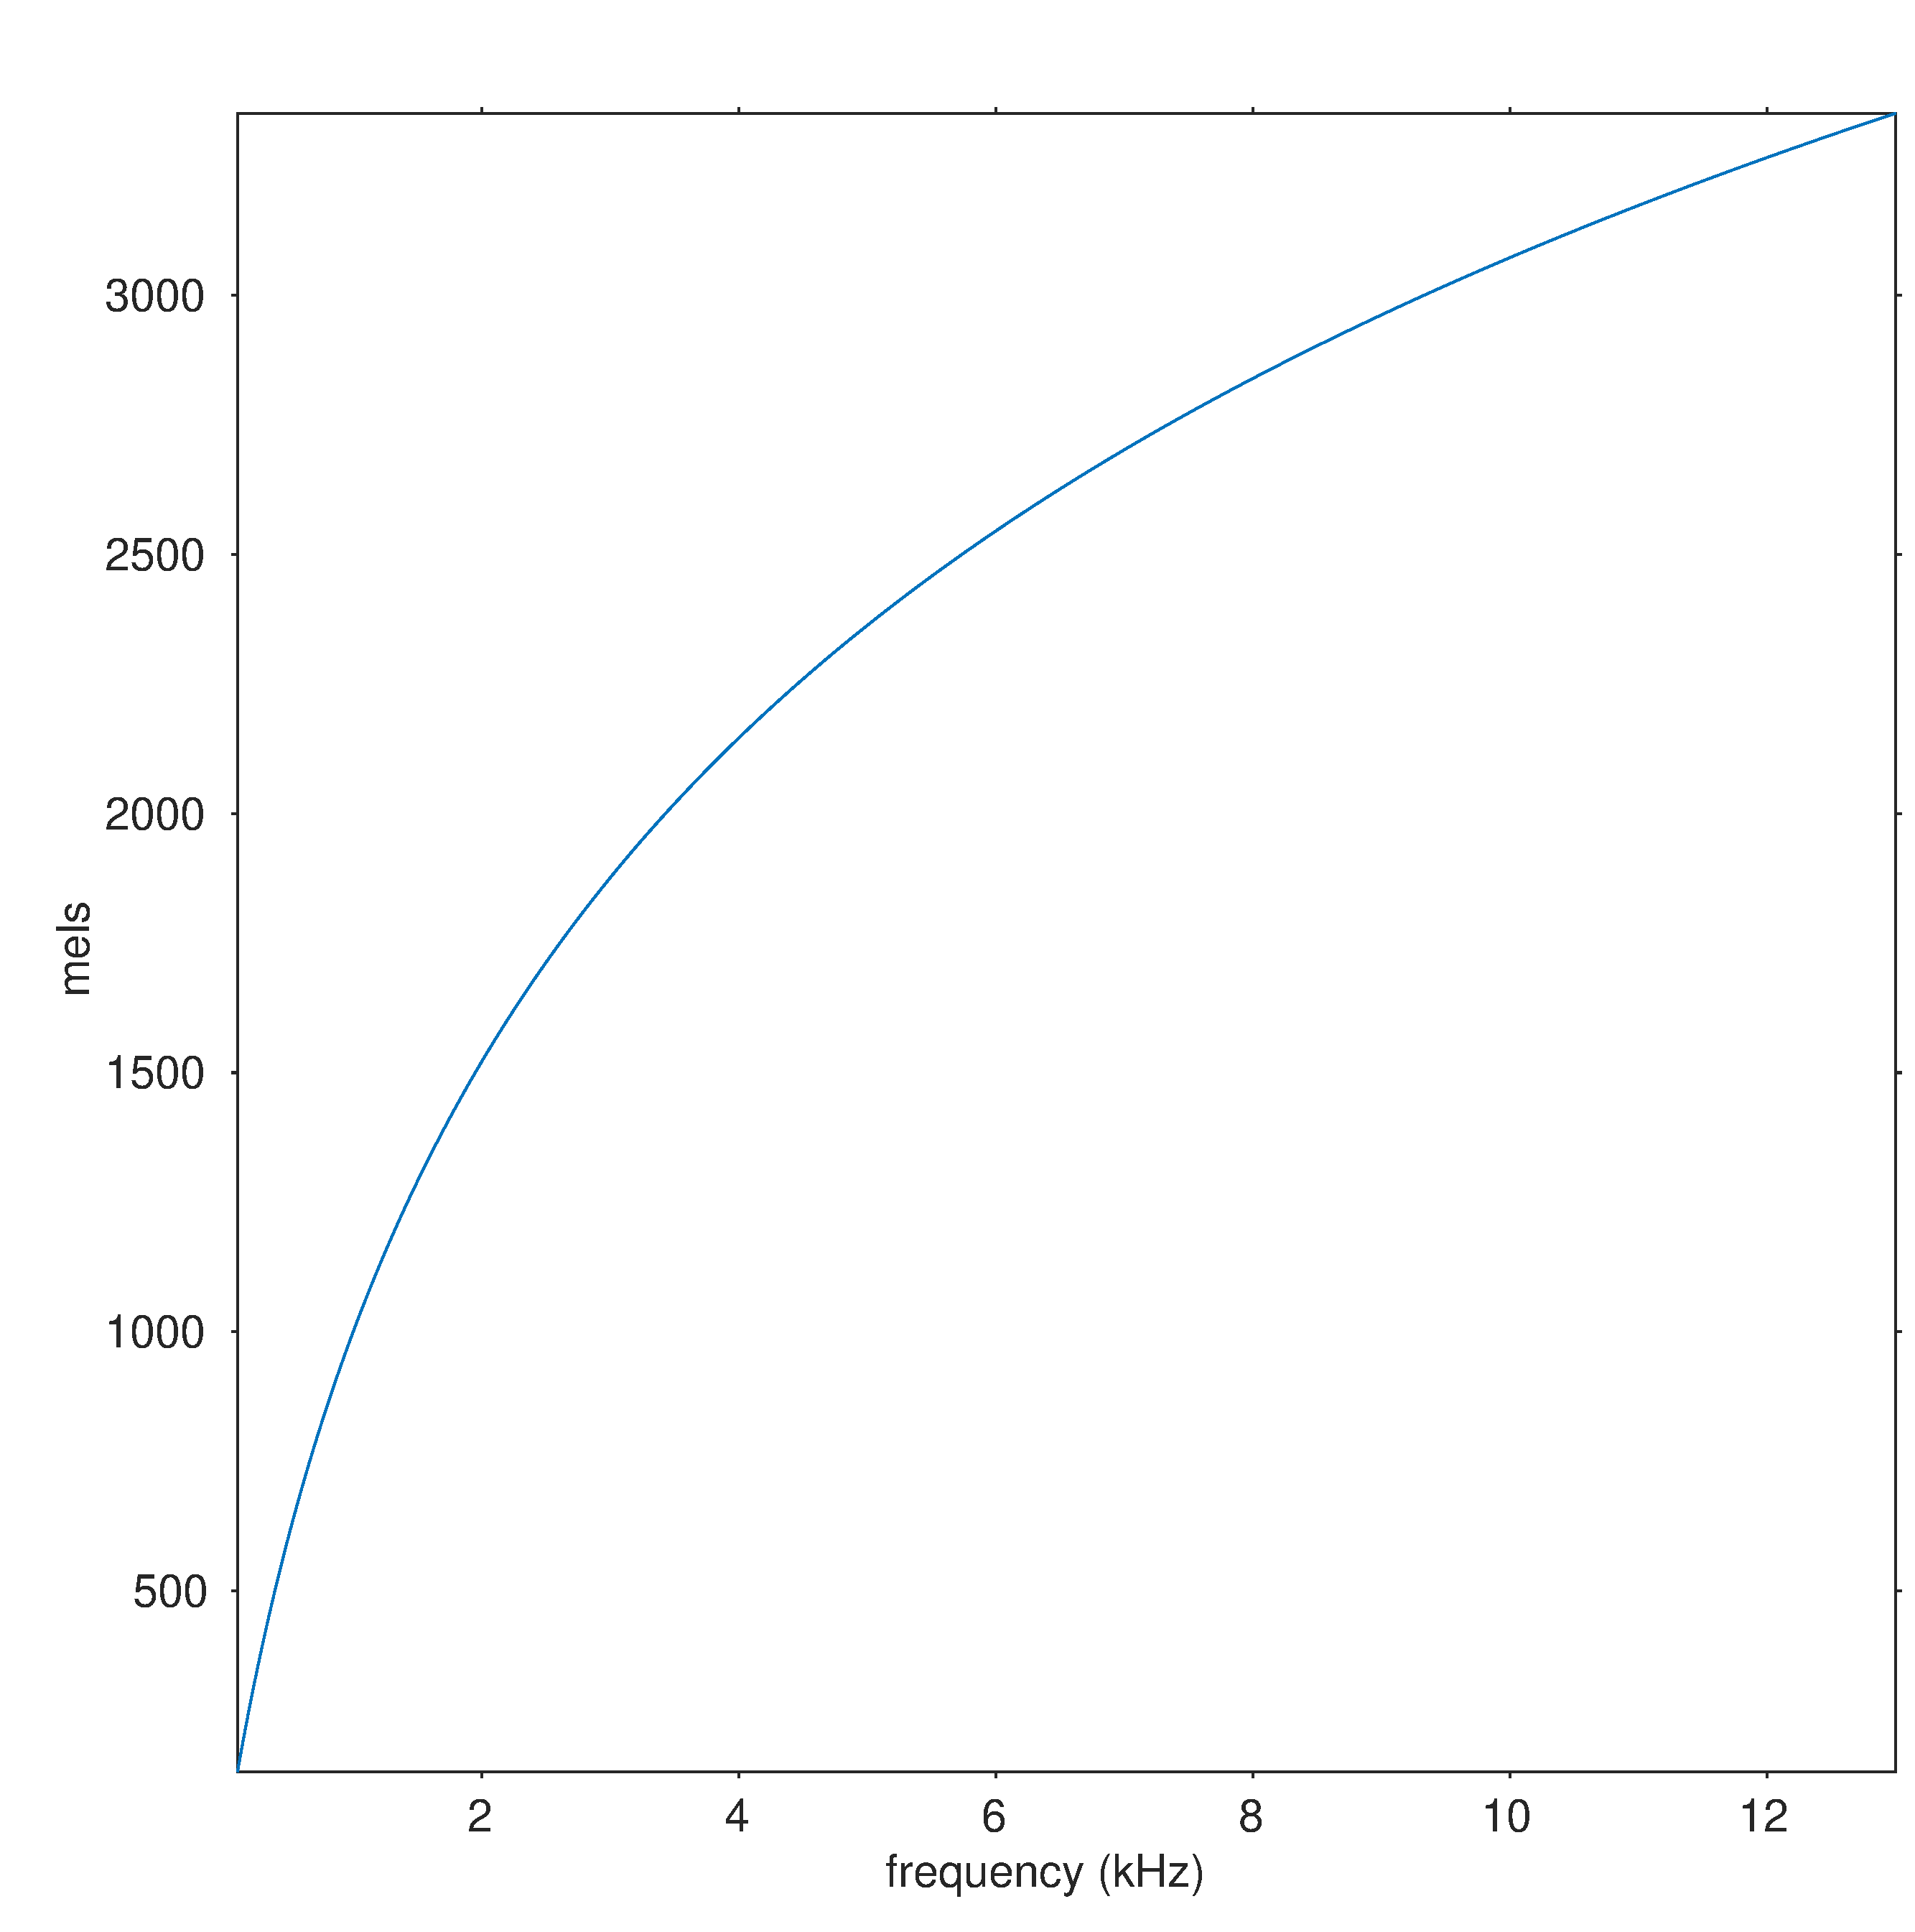
\includegraphics[width=\linewidth]{gfx/hz2mel.eps}
	\caption{The relationship between Hz and mels is logarithmic.}
	\label{fig:hz2mel}
\end{figure}

\begin{figure}[h]
	\centering
	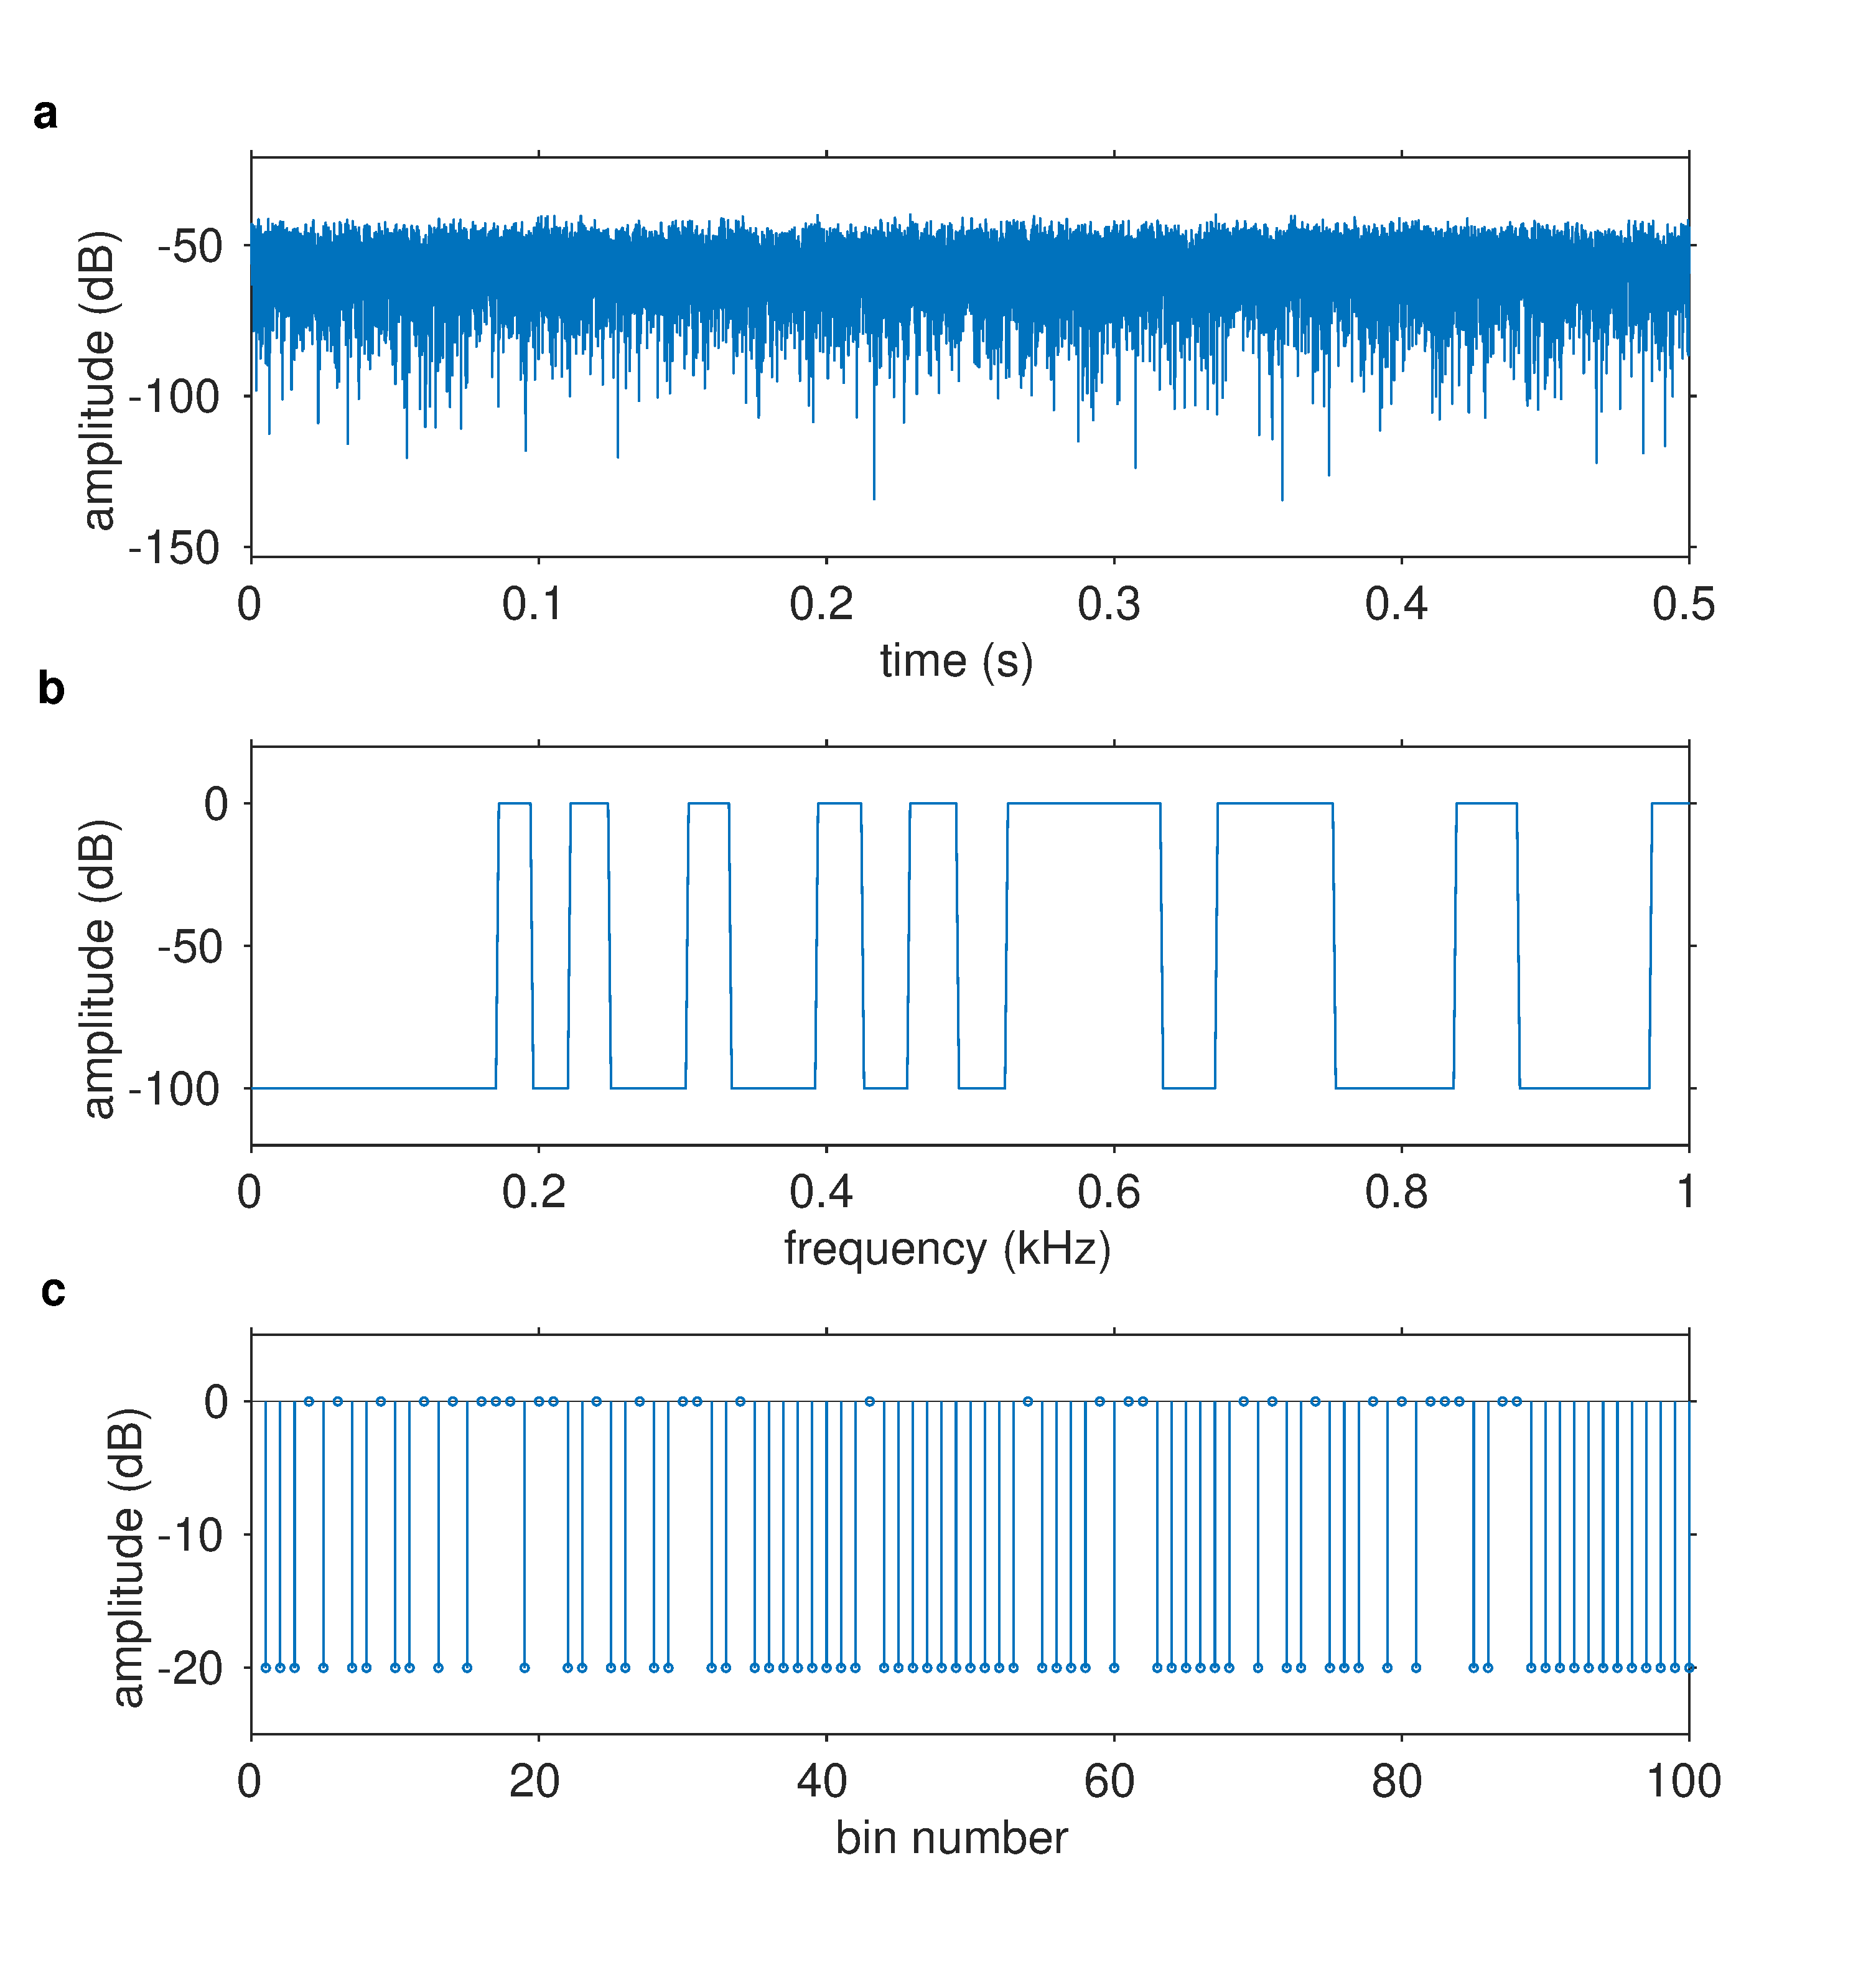
\includegraphics[width=\linewidth]{gfx/example_stimulus.eps}
	\caption{Example stimulus. \textbf{(a)} shows the waveform of the stimulus,
  \textbf{(b)} the frequency spectrum from which the waveform was generated,
  and \textbf{(c)} the $100$-dimensional bin representation.}
	\label{fig:examplestimulus}
\end{figure}

Furthermore, to reduce the system complexity by more than 80x,
we implement tonotopic binning, where the frequency scale is binned
along $100$ equally mel-spaced bins (Fig. \ref{fig:examplestimulus}).

\section{Hyperparameter Sweep}

To determine a suitable stimulus generation method,
we performed a hyperparameter sweep over
nine different stimulus generation methods.
We used an \textit{in-silico} model of the experiment,
with an artificial subject, but matched against American Tinnitus Association (ATA) tinnitus examples,
as in the human experiment.

The methods are as follows:

\begin{enumerate}
  \item \textit{Bernoulli}: A binned method in which each tonotopic bin
  has a probability $bin \_ prob$ of being set to $0$ dB otherwise it is set to $-20$ dB.
  \item \textit{Brimijoin}: A binned method inspired by \cite{brimijoinInternalRepresentationVowel2013}.
  Each bin is assigned an amplitude value chosen from a uniform distribution of discrete values
  on the interval $[-20, 0]$. We used $6$ steps, which is consistent with the original paper.
  \item \textit{Gaussian Noise No Bins}: The amplitude of each frequency was determined by
  Gaussian noise with known mean and variance, which are hyperparameters $amplitude \_ mean$ and $amplitude \_ var$.
  \item \textit{Gaussian Noise}: A binned method where the bin amplitudes were
  determined by a Gaussian random variable with known mean and variance, \eg $\mathcal{N}(amplitude \_ mean$ and $amplitude \_ var)$.
  \item \textit{Gaussian Prior}: A binned method where the number of filled bins
  was set by $\mathrm{round}(\mathcal{N}(n \_ bins \_ filled \_ mean, n \_ bins \_ filled \_ var))$,
  and that many bins were filled randomly at $0$ dB (unfilled bins were set to $-20$ dB).
  \item \textit{Power Distribution}: A binned method where the amplitude of each bin
  is drawn from a distribution matching the histogram of amplitudes
  of the American Tinnitus Association tinnitus examples from their website.
  \item \textit{Uniform Noise No Bins}: The amplitude associated with each frequency
  is determined by a uniform random variable on the interval $[-20, 0]$ dB.
  \item \textit{Uniform Noise}: The amplitude associated with each tonotopic bin
  is determined by a uniform random variable on the interval $[-20, 0]$ dB.
  \item \textit{Uniform Prior}: The number of filled bins is determined by drawing an integer
  from the discrete interval $[min \_ bins, max \_ bins] \in \mathbb{Z}^+$. Then, that many bins are set to $0$ dB,
  and all other bins are set to $-20$ dB. $min \_ bins$ and $max \_ bins$ are hyperparameters.
\end{enumerate}

9 methods and 8 hyperparameters were varied in the hyperparameter sweep grid search (Table \ref{tbl:hyperparameters}).
Methods were evaluated \textit{in-silico} using the model:

\begin{equation}
  y = \mathrm{sgn}(\Psi \bar{x})
\end{equation}

where $y \in \mathbb{R}^n$ is the binary response vector,
$\Psi \in \mathbb{R}^{n \times d}$ is the stimulus matrix,
and $\bar{x} \in \mathbb{R}^d$ is the true target signal (the spectrum of the ATA tinnitus example).

Each stimulus generation method, with different hyperparameters,
was evaluated for target signals: buzzing, electric, roaring, screeching, static, and tea kettle.

\begin{table}[ht]
	\begin{center}	
		\small
		\resizebox{1\columnwidth}{!}{
			\begin{tabular}{ m{0.35\columnwidth} m{0.5\columnwidth} b{0.15\columnwidth}}	
				\multicolumn{3}{c}{\textsc{Hyperparameters}} \\
				\hhline{===}
				{Name} & {Values} & Unit \\ 
				\hline
				n\textunderscore bins & 10, 30, 100, 200, 300 & n.d. \\
				bin\textunderscore prob & 0.1, 0.3, 0.5, 0.8 & n.d. \\
                amplitude\textunderscore mean & -35 & dB \\
                amplitude\textunderscore var & 5, 10, 20 & $\sqrt{\mathrm{dB}}$ \\
                n\textunderscore bins\textunderscore filled \textunderscore mean & 1, 3, 10, 20, 30 & n.d. \\
                n\textunderscore bins\textunderscore filled\textunderscore var & 0.01, 1, 3, 10 & n.d. \\
                min\textunderscore bins & 1, 3, 10, 20, 30 & n.d. \\
                max\textunderscore bins & 10, 20, 30, 50 & n.d. \\
				\hhline{===}
			\end{tabular}
		}
	\end{center}
%\normalsize
	\caption{Hyperparameter values tested in the parameter sweep. Not all methods use all hyperparameters,
    and some combinations of hyperparameters are invalid (\eg when $min\_ bins > max \_ bins$).
    n.d. means ``non-dimensional'' and refers to a unitless number.
    }
	\label{tbl:hyperparameters}
\end{table}

Reconstructions were computed using linear regression and compressed sensing
(\cf the main paper)
and reconstruction accuracy was measured using Pearson's $r^2$ vs. the target signal.

Fine-tuning of parameters proceeded iteratively,
bearing in mind both the performance of the stimulus generation methods
in the \textit{in-silico} experiment as well as computational efficiency,
qualitative distinguishability of stimuli from each other by a human listener,
and viability of compressed sensing as an efficiency enhancement.
This process resulted in $n \_ bins$ being fixed to $100$ and
the number of trials in the \textit{in-silico} experiment being set to $1000$.

\begin{table}[ht]
	\begin{center}	
		\small
		\resizebox{1\columnwidth}{!}{
			\begin{tabular}{l S[table-format=12.2] S[table-format=12.2] S[table-format=12.2] S[table-format=6.2] S[table-format=6.2] S[table-format=6.2] S[table-format=6.2]}	
				\multicolumn{7}{c}{\textsc{Hyperparameter Sweep Results}} \\
				\hhline{=======}
				Stimulus Type & n \_ bins \_ filled \_ mean & n \_ bins \_ filled \_ var & min \_ bins & max \_ bins & CS \_ r^2 & LR \_ r^2 \\ 
				\hline
				Gaussian Prior    & 20 & 1 & & & 0.83 & 0.86 \\
        Uniform Prior     & & & 30 & 30 & 0.82 & 0.86 \\
        Uniform Prior     & & & 20 & 20 & 0.82 & 0.86 \\
        Gaussian Prior    & 20 & 1 & & & 0.82 & 0.86 \\
        Gaussian Prior    & 12 & 0.01 & & & 0.81 & 0.83 \\
				\hhline{=======}
			\end{tabular}
		}
	\end{center}
%\normalsize
	\caption{Top-5 stimulus generation methods by $r^2$ score averaged over
  buzzing, electric, roaring, screeching, and static tinnitus examples,
  with $n \_ bins = 100$ and $n \_ trials = 1000$.
  }
	\label{tbl:hparam_results}
\end{table}

%       stimuli_type       n_bins_filled_mean    n_bins_filled_var    min_bins    max_bins    mean_r2_cs    mean_r2_linear
%     _________________    __________________    _________________    ________    ________    __________    ______________

%     {'GaussianPrior'}            20                  0.01             NaN         NaN          0.83            0.86     
%     {'UniformPrior' }           NaN                   NaN              30          30          0.82            0.86     
%     {'UniformPrior' }           NaN                   NaN              20          20          0.82            0.86     
%     {'GaussianPrior'}            20                     1             NaN         NaN          0.81            0.86     
%     {'GaussianPrior'}            10                  0.01             NaN         NaN          0.81            0.83     
%     {'GaussianPrior'}            30                     1             NaN         NaN           0.8            0.84     
%     {'UniformPrior' }           NaN                   NaN              10          10           0.8            0.83     
%     {'GaussianPrior'}            10                     1             NaN         NaN          0.79            0.83     
%     {'UniformPrior' }           NaN                   NaN              20          30          0.79            0.79     
%     {'GaussianPrior'}            30                  0.01             NaN         NaN          0.79            0.86     


Table \ref{tbl:hparam_results} shows the top 5 best-performing methods
in the \textit{in-silico} experiment.
Gaussian Prior and Uniform Prior outperform all other methods,
with 10-30\% of bins being filled.
The variance of the number of filled bins for top-performing methods
is extremely low.
Due to rounding to the nearest integer, a Gaussian Prior method with very low variance
converges to a Uniform Prior method with equal min and max bin parameters.
In the main paper, we used the Uniform Prior method with 30 filled bins ($min \_ bins = max \_ bins = 30$).

\section{Sparsity of ATA Tinnitus Examples}

A necessary condition for compressed sensing to produce reconstructions results
beyond the Shannon-Nyquist limit is that the signal to be reconstructed is sparse in some basis
\cite{taghoutiCompressedSensing2020}.
A signal is considered to be at least $k$ sparse when it has at most $k$ nonzero elements.
A signal is considered $k$-sparse under some basis, when a basis-transformed version
of that signal is $k$-sparse.
Here we show that the 8,193-dimensional ATA example tinnitus spectra are sparse under
the discrete cosine basis.
The signal representation in the basis is produced by computing its discrete cosine transform (DCT).
We computed the DCT of each ATA example spectrum
and set all but the top 32 DCT-frequencies to zero
before taking the inverse transform back to the Fourier domain.
Figure \ref{fig:target_signal_sparsity_1}
shows that while some high-frequency information was lost,
that the 32-sparse signal preserves the salient information of the signal.
The tonotopic bin representation is also sparse under the discrete cosine basis
(Fig. \ref{fig:target_signal_sparsity_2}).
The sparsity value $k=32$ was chosen by examining the decay of the sorted power spectrum
of the tinnitus Fourier spectra in the discrete cosine basis (Fig. \ref{fig:target_signal_sparsity_3}).
We see that the power of the signal rapidly decays after only a few DCT-frequencies.

\begin{figure}[h]
	\centering
	\includegraphics[width=\linewidth]{gfx/target_signal_sparsity_1.eps}
	\caption{Tinnitus signals are approximately sparse.
    Each subfigure plots the true spectrum of an ATA tinnitus example
    in blue (8,193 nonzero dimensions) and a 32-sparse (32 non-zero dimensions)
    approximation in green.
    The sparse signal is a low-pass filtered version of the original signal
    that retains the salient dynamics.
    \textbf{(a)} through \textbf{(f)} correspond to
    buzzing, electric, roaring, static, tea kettle, and screeching ATA examples
    respectively.}
	\label{fig:target_signal_sparsity_1}
\end{figure}

\begin{figure}[h]
	\centering
	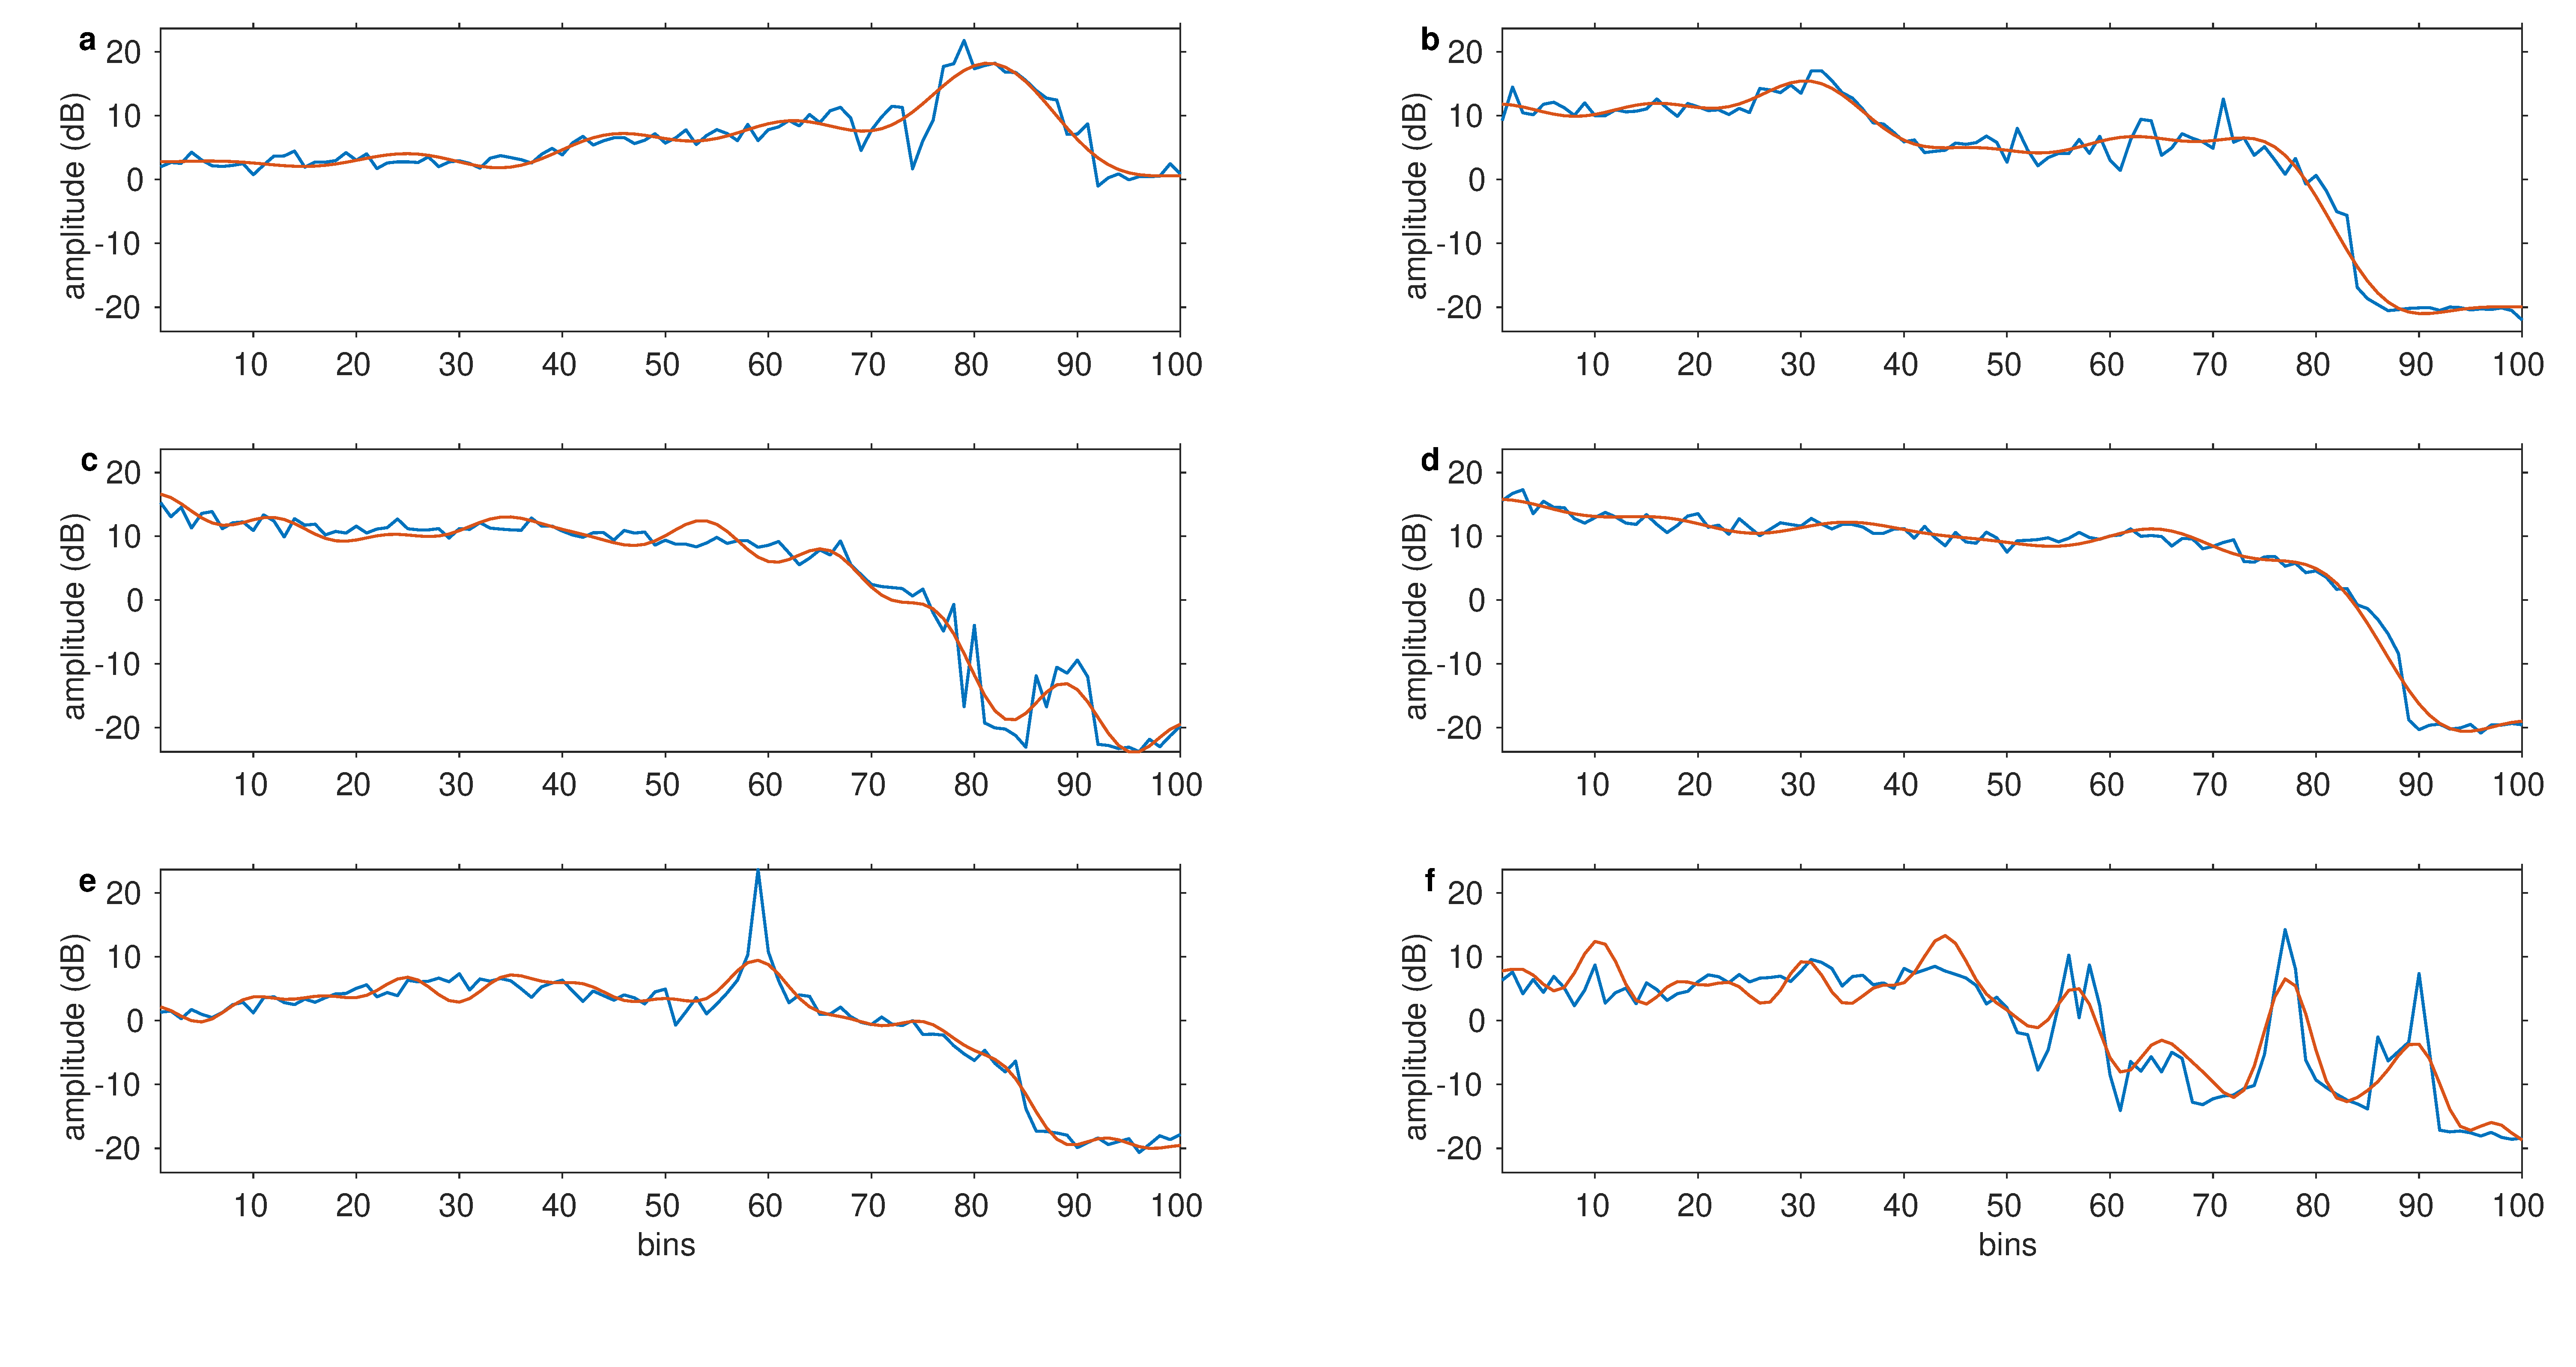
\includegraphics[width=\linewidth]{gfx/target_signal_sparsity_2.eps}
	\caption{Tonotopic bin representations of tinnitus signals are approximately sparse
    in the DCT basis.
    Each subfigure plots the tonotopic bin representation of an ATA tinnitus spectrum
    in blue (100 nonzero dimensions) and the bin representation of a 10-sparse
    approximation in red (10 nonzero dimensions).
    The sparse signal is a low-pass filtered version of the original signal
    that retains the salient dynamics.
    \textbf{(a)} through \textbf{(f)} correspond to
    buzzing, electric, roaring, static, tea kettle, and screeching ATA examples
    respectively.}
	\label{fig:target_signal_sparsity_2}
\end{figure}

\begin{figure}[h]
	\centering
	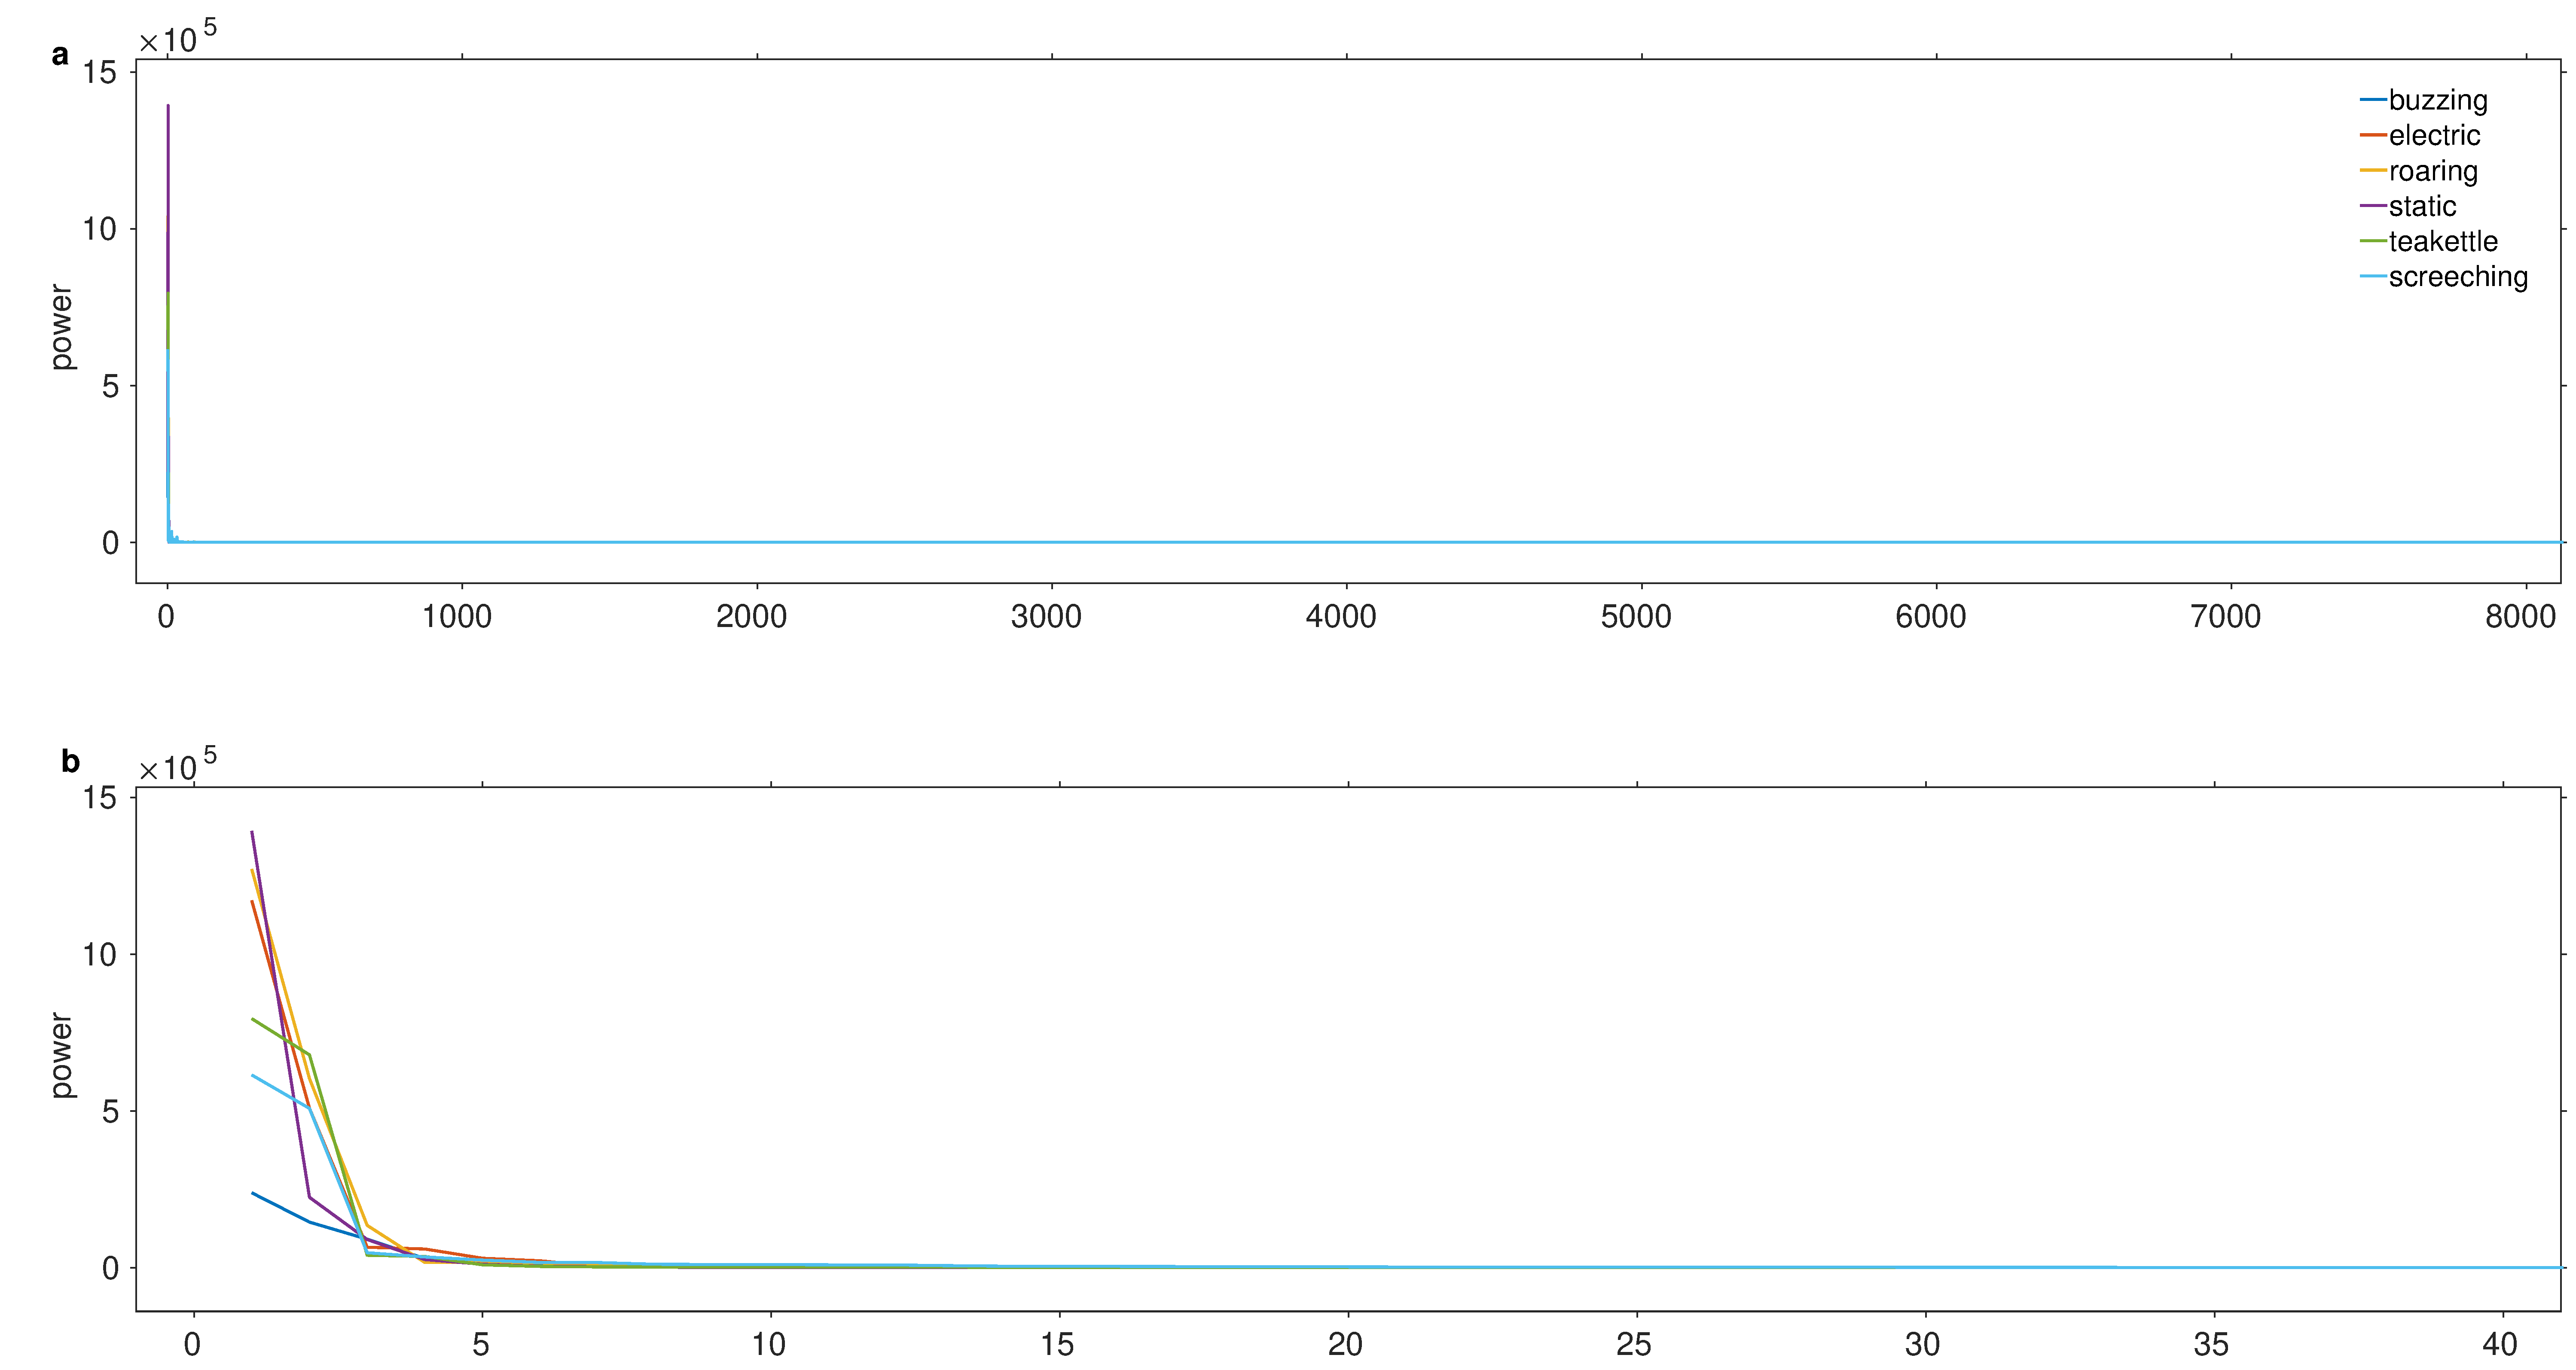
\includegraphics[width=\linewidth]{gfx/target_signal_sparsity_3.eps}
	\caption{DCT-transformed tinnitus spectra have high power in a few frequencies
  and low power elsewhere. \textbf{a} shows the power spectrum of DCT-transformed
  ATA tinnitus example Fourier spectra. \textbf{b} shows the highest 40 DCT frequencies
  in ranked order, illustrating a sharp decay to zero, indicating sparsity
  of tinnitus spectra in the DCT basis.}
	\label{fig:target_signal_sparsity_3}
\end{figure}

\FloatBarrier

\bibliographystyle{IEEEtran}
\bibliography{IEEEabrv,../paper/mybib}

% that's all folks
\end{document}



